\section{Graph Theory}
Before we begin with formal definitions, let us start with an example. Suppose we have a group of people and some of them are friends. We may represent these by drawing a point for each person, and a line for each friendship. Obviously, the position of the dots and lines does \emph{not} matter, just the connections.

\begin{definition}
    A \emph{graph} $G$ consists of two finite sets:
    \begin{itemize}
        \item a non-empty set $V(G)$ of vertices, and
        \item a (possibly empty) set $E(G)$ of edges, where each edge is associated with a set $\left\{v,w\right\}\subseteq V(G)$
    \end{itemize}

    The vertices $v$ and $w$ are called the end points of the edge.
\end{definition}

\begin{example}
    \begin{figure}[H]
        \centering
        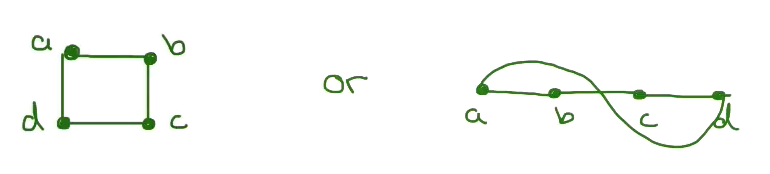
\includegraphics[width=0.5\textwidth]{basic_graph}
    \end{figure}

    This graph $G$ has $V(G) = \left\{a,\,b,\,c,\,d\right\}$ and has $4$ edges whose endpoints are $$\left\{a,\,b\right\},\,\left\{b,\,c\right\},\,\left\{c,\,d\right\},\,\left\{a,\,d\right\}$$
\end{example}

\begin{definition}
    A \underline{loop} is an edge wose endpoints are equal, which is denoted $\{v,\,v\}$ or $\{v\}$
\end{definition}

\begin{definition}
    \underline{Parallel edges} (or \underline{multiple edges}) are two or more edges with the same set of endpoints.
\end{definition}

\begin{definition}
    A \underline{simple graph} is a graph with no loops or parallel edges.

    \begin{figure}[H]
        \centering
        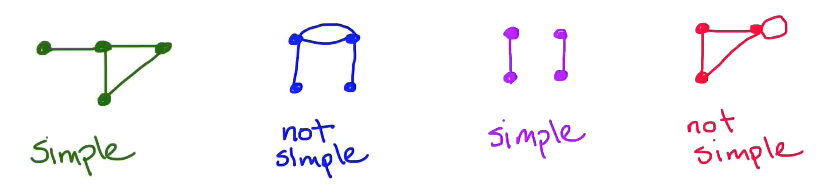
\includegraphics[width=0.5\textwidth]{simplicity}
    \end{figure}
\end{definition}

\begin{example}
    Referred to below.
    \begin{figure}[H]
        \centering
        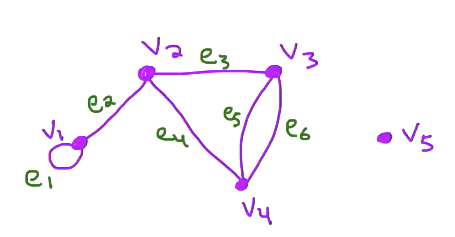
\includegraphics[width=0.5\textwidth]{example_graph_for_defs}
    \end{figure}
\end{example}

\begin{definition}
    An edge and a vertex are \underline{incident} if and only if the vertex is an endpoint of the edge.
    \\ \\
    Ex. $e_3$ is incident with $v_2$ and $v_3$. $v_1$ is incident with $e_1$ and $e_2$.
\end{definition}

\begin{definition}
    Two edges are \underline{adjacent} if they are incident with the same vertex.

    The vertices are \underline{adjacent} if they are connected by an edge (ie there is an edge they are both incident with).
    \\ \\
    Ex. $e_2$ and $e_3$ are adjacent. $v_2$ and $v_4$ are adjacent. $v_1$ and $v_4$ are non-adjacent.
\end{definition}

\begin{definition}
    An \underline{isolated} vertex is a vertex which is incident with no edges. Namely, $v_5$ above.
\end{definition}

\begin{definition}
    The \underline{degree} of a vertex $v$ is the number of edges indcident with $v$, where we count each loop \emph{twice}. We write this as $\text{deg}(v)$.
\end{definition}

\begin{theorm}
    \underline{The Handshake Theorm}

    Let $G$ be a graph with $n$ vertices $$V(G) = \left\{v_1,\,v_2,\,v_3,\,\dots,\,v_n\right\}$$

    Then $$\sum_{i=1}^n \text{deg}(v_i) = \text{deg}(v_1) + \text{deg}(v_2) + \dots + \text{deg}(v_n) = 2 \cdot |E(G)|$$
\end{theorm}

\subsection{Getting Between Vertices}
Let $G$ be graph and let $v$ and $w$ be vertices in $G$. A \emph{walk} from $v$ to $w$ is a finite alternating sequence 
\begin{equation}
    v_0 e_1 v_1 e_2 \dots v_{n-1}e_n v_n
\end{equation}

of vertices and edges where $v_0 = v$, $v_n = w$, and $e_i$ is an edge with endpoints $\left\{v_{i-1},\,v_i\right\}$ for $i\in\left\{1,\,\dots,\,n\right\}$

\begin{example}
    \begin{figure}[H]
        \centering
        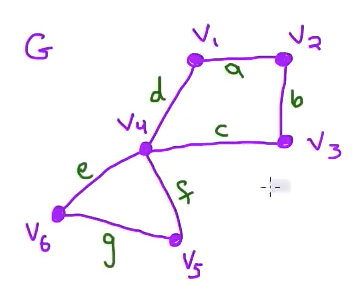
\includegraphics[width=0.25\textwidth]{walk}
    \end{figure}
    $v_5 f v_4 c v_3 c v_4 e v_6$ is a walk from $v_5$ to $v_6$.

    Also, $v_5 g v_6$ is a walk from $v_5$ to $v_6$.
\end{example}

\begin{definition}
    A graph $G$ is \underline{connected} if and only if, given any two vertices $v$ and $w$ in $G$, there is a walk from $v$ to $w$.

    A \underline{trail} is a walk whose edges are distinct.

    A \underline{circuit} is a trail that starts and ends at the same vertex.
\end{definition}

\begin{definition}
    Let $G$ be a graph. An \underline{Euler circuit} for $G$ is a circuit that contains every edge of $G$ exactly once.

    Lemma: if a graph $G$ has an Euler circuit, then each vertex has even degree. Proof in lec 35.
\end{definition}

\begin{theorm}
    Let $G$ be a connected graph. Then $G$ has an Euler circuit if and only if every vertex of $G$ has even degree.
\end{theorm}

\begin{definition}
    Let $G$ be a graph and let $u,\, v \in V(G)$. An \underline{Euler trail} from $u$ to $v$ is a trail from $u$ to $v$ that uses every edge exactly once.
\end{definition}
\begin{theorm}
    Let G be a connected graph and let \(u, v\in v(G)\).\\
    If \(u = v\) then G has an Euler trail from u to v if and only if every vertex of G has even degree.\\
    If \(u \neq v\) then G has an Euler trail from u to v iff u and v have odd degree and all other vertices have even degree.
\end{theorm}


